\subsection{Universidad de Oxford}

Este experimento corresponde a la Universidad de Oxford, ubicada en Inglaterra, cuyo dominio web es \url{www.ox.ac.uk}.

\begin{figure}[H]
    \centering
    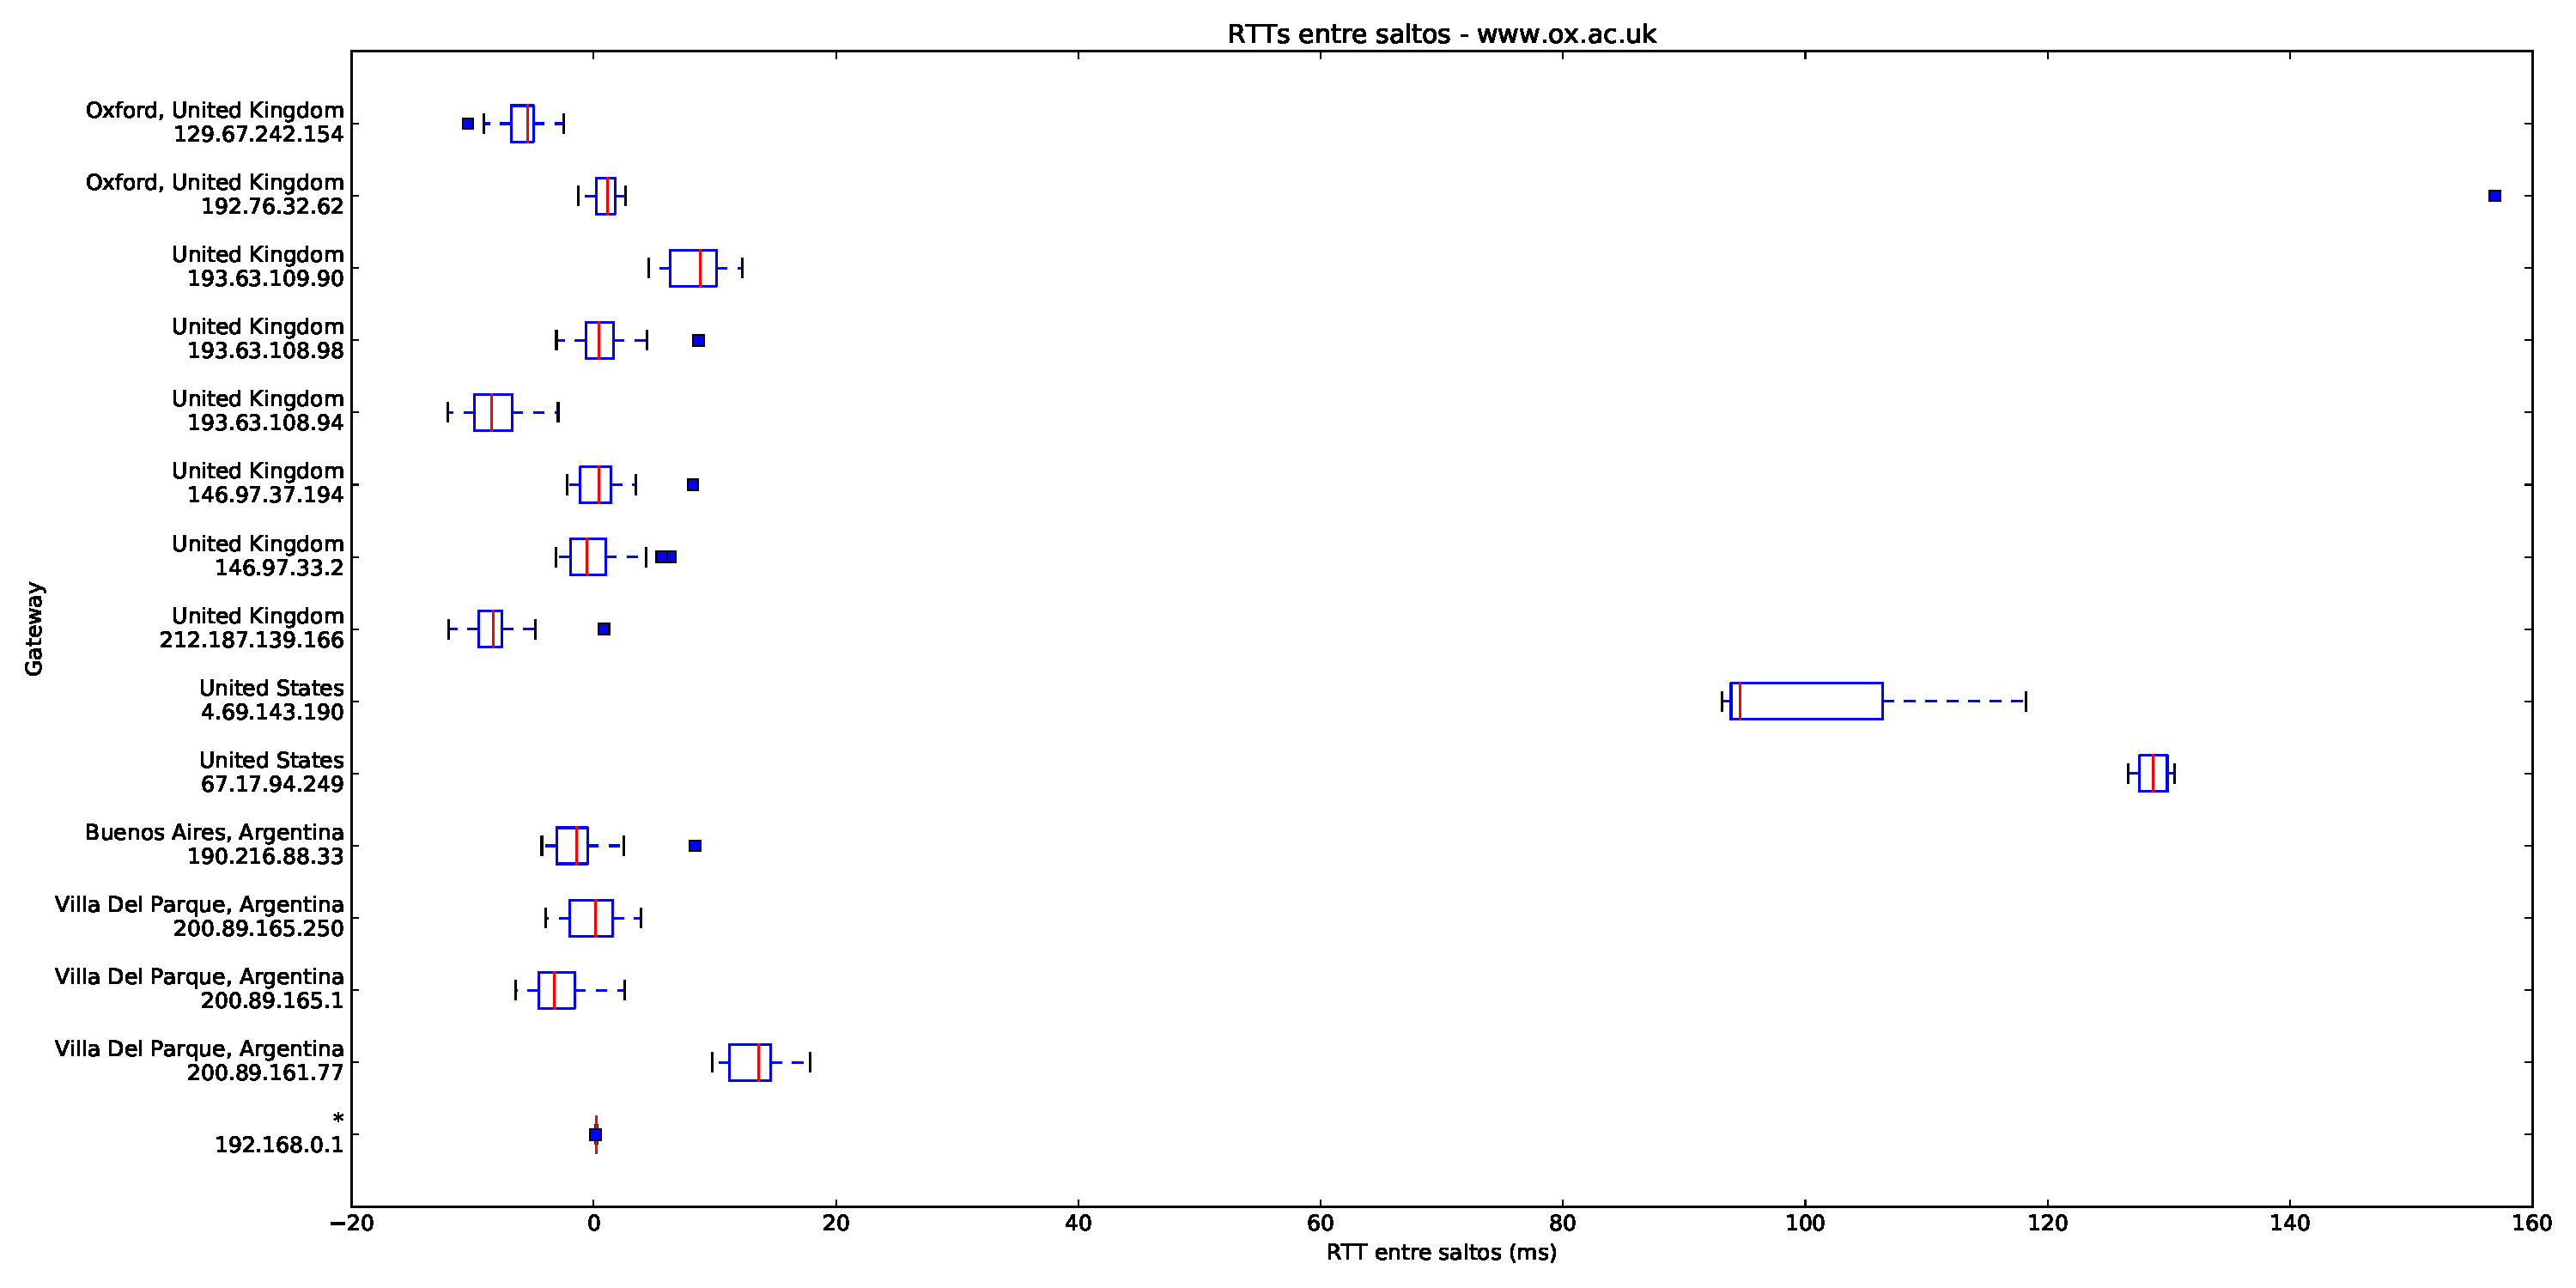
\includegraphics[width=8.5cm]{img/grafico1-www-ox-ac-uk.pdf}
    \caption{\normalfont RTTs entre saltos. El valor asignado al $i$-ésimo nodo corresponde al salto entre el $i$-ésimo y el $i - 1$-ésimo nodo. Para el primer nodo se utiliza simplemente su RTT.}
\end{figure}

\begin{figure}[H]
    \centering
    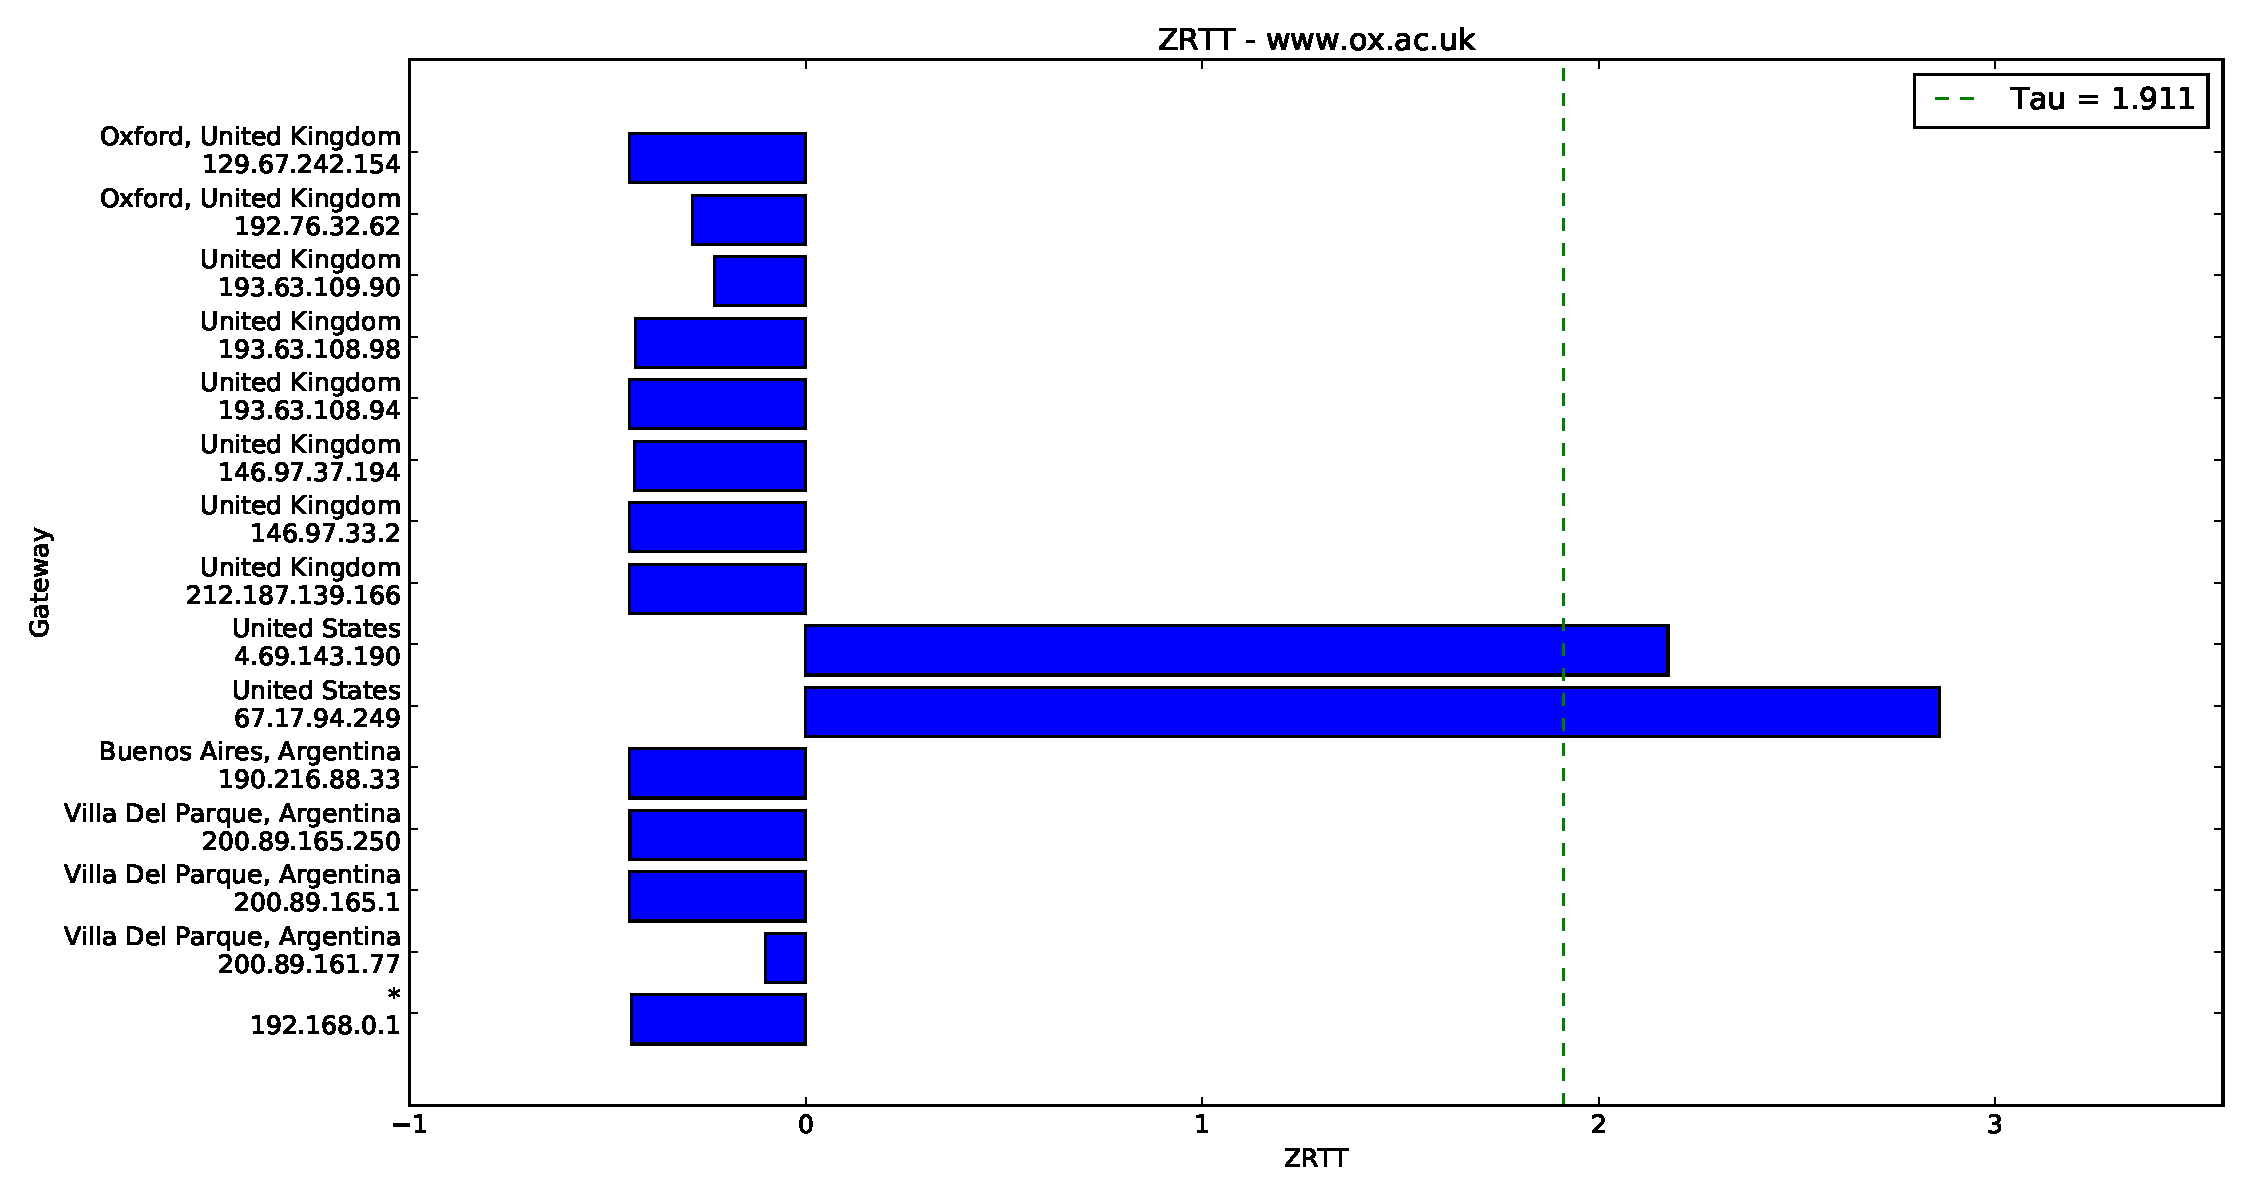
\includegraphics[width=8.5cm]{img/grafico2-www-ox-ac-uk.pdf}
    \caption{\normalfont ZRTTs entre saltos.}
\end{figure}

\begin{figure}[H]
    \centering
    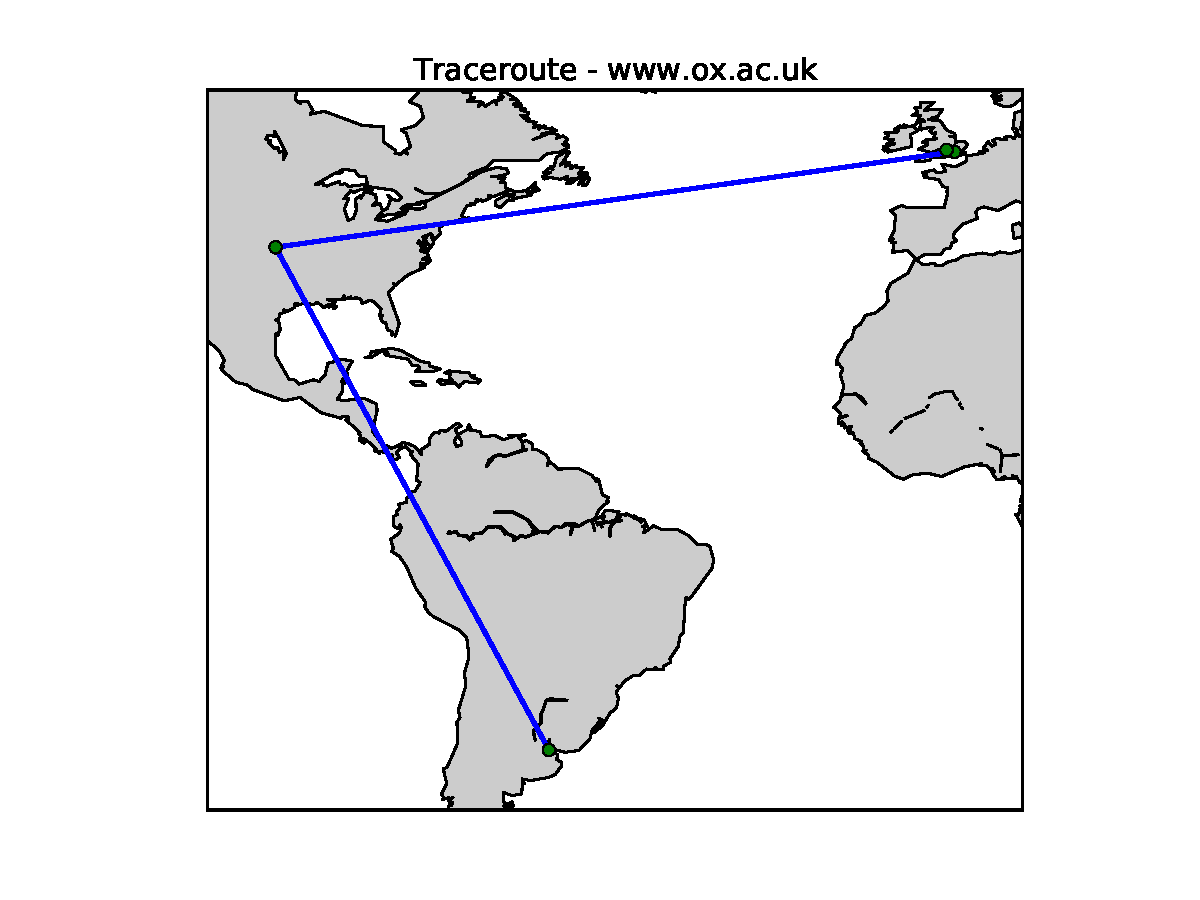
\includegraphics[width=8.5cm]{img/grafico3-www-ox-ac-uk.pdf}
    \caption{\normalfont Ubicación geográfica estimada de la ruta tomada.}
\end{figure}

Al realizar el traceroute, el porcentaje de saltos que no respondió los time exceeded fue de 28.57\% (exactamente 6 de 21). En términos de saltos que sí responden, la ruta tiene 15 nodos, incluyendo el router correspondiente a la red desde la cual se realizó el experimento.

Como se ve en los gráficos, se pueden observar dos \textit{outlier} entre los saltos efectuados, correspondientes a los enlaces entre Argentina - Estados Unidos y Estados Unidos - Inglaterra. Efectivamente, estos son los únicos dos enlaces intercontinentales que se encuentran entre el origen y el destino, y nuestro modelo pudo detectarlos. Al igual que en varios de nuestros experimentos, los paquetes pasan por Estados Unidos para llegar a destino.

Además, se puede observar en el gráfico de las ubicaciones geográficas que en el camino hasta llegar hasta la Universidad de Oxford, el paquete pasa por otra ciudad ubicada en Inglaterra. Luego de varios experimentos con otras universidades cercanas, podemos predecir que esta ciudad se trata de Londres, donde, efectivamente, se encuentra un enlace submarino con Estados Unidos.
